
%%% Local Variables: 
%%% mode: latex
%%% TeX-master: "../lec02"
%%% End: 

\section{Operações para tomada de decisões}

\begin{frame}{Desvios}
\vspace{-0.25cm}
\begin{block}{Desvio de fluxo}
  \begin{itemize}
  \item {\bf beq} registro1, registro2, R1
    \begin{quote}
      { Desvia o fluxo das instruções para o rótulo R1 se o conteúdo do
      registro1 for \alert{igual} ao do registro2.}
    \end{quote}
  \item {\bf bne} registro1, registro2, R1
    \begin{quote}
      { Desvia o fluxo das instruções para o rótulo R1 se o conteúdo do
      registro1 for \alert{diferente} ao do registro2.}
    \end{quote}
  \end{itemize}
\end{block}
\end{frame}

\begin{frame}{Desvio de fluxo}{Exemplo}
\begin{block}{Exemplo de desvio de fluxo}
  \$s0 $\leftarrow$ f, \$s1 $\leftarrow$ g, \$s2 $\leftarrow$ h, \$s3
  $\leftarrow$ i, \$s4 $\leftarrow$ j\\
  \smallskip
  código em C:\\
  \begin{tt}
    \hspace{0.5cm} if (i == j) f = g + h; else f = g - h;\\
  \end{tt}
  \bigskip
  Instruções MIPS:
\begin{tabbing}
  \hspace{1cm}\=\hspace{1cm}\= bne \=\$s3, \$s4, Else\\
  \>\>add \$s0, \$s1, \$s2\\
  \>\>j \>Exit\\
  \>Else:\> sub \$s0, \$s1, \$s2 \\
  \>Exit:\\
\end{tabbing}

\end{block}

\end{frame}

\section{Formato das instruções}

\begin{frame}{Formato básico das instruções MIPS}{Formato I}

  \def\mywidth{1.75cm}
  \def\myheight{0.75cm}

\begin{block}{Formato I ({\em immediate})}
  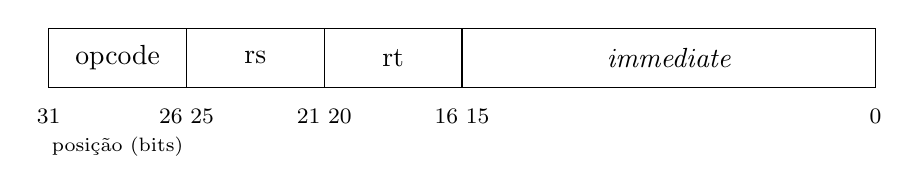
\begin{tikzpicture}
    \foreach \x/\field/\pos in {0/opcode/31,1/rs/{26 25},2/rt/{21
        20}} {
      \draw (\x*\mywidth,0) rectangle (\x*\mywidth+\mywidth,\myheight);
      \node at (\x*\mywidth+\mywidth/2, \myheight/2) {\field};
      \node at (\x*\mywidth, -\myheight/2) {\footnotesize\pos};
    }
    \draw (3*\mywidth,0) rectangle (6*\mywidth,\myheight);
    \node at (4*\mywidth+\mywidth/2, \myheight/2) {\em immediate};
    \node at (3*\mywidth, -\myheight/2) {\footnotesize 16 15};

    \node at (6*\mywidth, -\myheight/2) {\footnotesize 0};
    \node at (\mywidth/2, -\myheight) {\scriptsize posição (bits)};
\end{tikzpicture}
\smallskip
\hrule
\bigskip
Exemplo:\\

\begin{tt}
  \hspace{2cm} lw \$t0, 32(\$t1)\\
\end{tt}
{\small\color{gray} \# lw -- opcode, rs $\leftarrow$ \$t1, rt
  $\leftarrow$ \$t0, {\em immediate} $\leftarrow$ 32}\\
\bigskip
  \begin{tikzpicture}
    \foreach \x/\field/\nbits/\ndec in
    {0/\only<1>{100011}/op - 6/\only<2>{\dec{35}},1/\only<1>{10010}/\$t1 -
      5/\only<2>{\dec{9}},2/\only<1>{01000}/\$t0 - 5/\only<2>{\dec{8}}} {
      \draw (\x*\mywidth,0) rectangle (\x*\mywidth+\mywidth,\myheight);
      \node at (\x*\mywidth+\mywidth/2, \myheight/2) {\field\ndec};
      \node at (\x*\mywidth+\mywidth/2, -\myheight/2) {\footnotesize\nbits{} bits};
    }
    \draw (3*\mywidth,0) rectangle (6*\mywidth,\myheight);
    \node at (4*\mywidth+\mywidth/2, \myheight/2) {\only<1>{0000
        0000 0010 0000}\only<2>{\dec{32}}};
    \node at (4*\mywidth+\mywidth/2, -\myheight/2) {\footnotesize 16 bits};
\end{tikzpicture}

\end{block}  

\end{frame}


\begin{frame}{Formato básico das instruções MIPS}{Formato J}

  \def\mywidth{1.75cm}
  \def\myheight{0.75cm}

\begin{block}{Formato J ({\em jump})}
  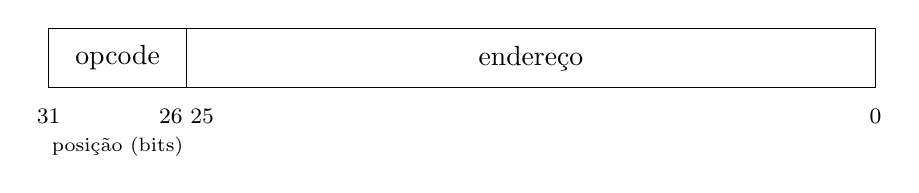
\begin{tikzpicture}
    \draw (0,0) rectangle (\mywidth,\myheight);
    \node at (\mywidth/2, \myheight/2) {opcode};
    \node at (0, -\myheight/2) {\footnotesize 31};
    
    \draw (\mywidth,0) rectangle (6*\mywidth,\myheight);
    \node at (3*\mywidth+\mywidth/2, \myheight/2) {endereço};
    \node at (\mywidth, -\myheight/2) {\footnotesize 26 25};

    \node at (6*\mywidth, -\myheight/2) {\footnotesize 0};
    \node at (\mywidth/2, -\myheight) {\scriptsize posição (bits)};
\end{tikzpicture}
\smallskip
\hrule
\bigskip
Exemplo:\\

\begin{tt}
  \hspace{2cm} j Exit\\
\end{tt}
{\small\color{gray} \# j -- opcode, Exit -- rótulo (endereço)}\\
\bigskip
  \begin{tikzpicture}
    \draw (0,0) rectangle (\mywidth,\myheight);
    \node at (\mywidth/2, \myheight/2) {\only<1>{000010}\only<2>{\dec{2}}};
    \node at (\mywidth/2, -\myheight/2) {\footnotesize op - 6 bits};
      
      \draw (\mywidth,0) rectangle (6*\mywidth,\myheight);
      \node at (3*\mywidth+\mywidth/2, \myheight/2) {\only<1>{00 0000 0000 0000
          0100 1011 0000}\only<2>{\dec{1200}}};
      \node at (3*\mywidth+\mywidth/2, -\myheight/2) {\footnotesize 26 bits};
\end{tikzpicture}

\end{block}  

\end{frame}


\def\thissection{Exercícios III}
\section{\thissection}

\def\mem{{\footnotesize\color{gray}\# (M)}}
\begin{frame}{\thissection}
  \large
  \begin{itemize}
  
  \item Desvios
    \begin{enumerate}
    \item {\tt if (a == b) a = a + 10; else b = b + 10;}
    \item {\tt for(i=0; i<10; i++) s[i] = 2+i;} \mem
    \end{enumerate}

  \end{itemize}

\end{frame}


\begin{frame}{TODO}
  
  \begin{itemize}
  \item loops
  \item MARS
  \item tabela mips
  \end{itemize}

\end{frame}

